\chapter{La metodologia}
In questo capitolo esporremo la metodologia utilizzata per la classificazione dei file audio, nello specifico partiremo dai software e i tipi di dati utilizzati per poi muverci verso l'estrazione delle feature la generazione dei dataset e la classificazione attraverso una particolare tecnica di machine learning chiamata multiple instance learning (MIL). 
\begin{figure}[h]
\centering
    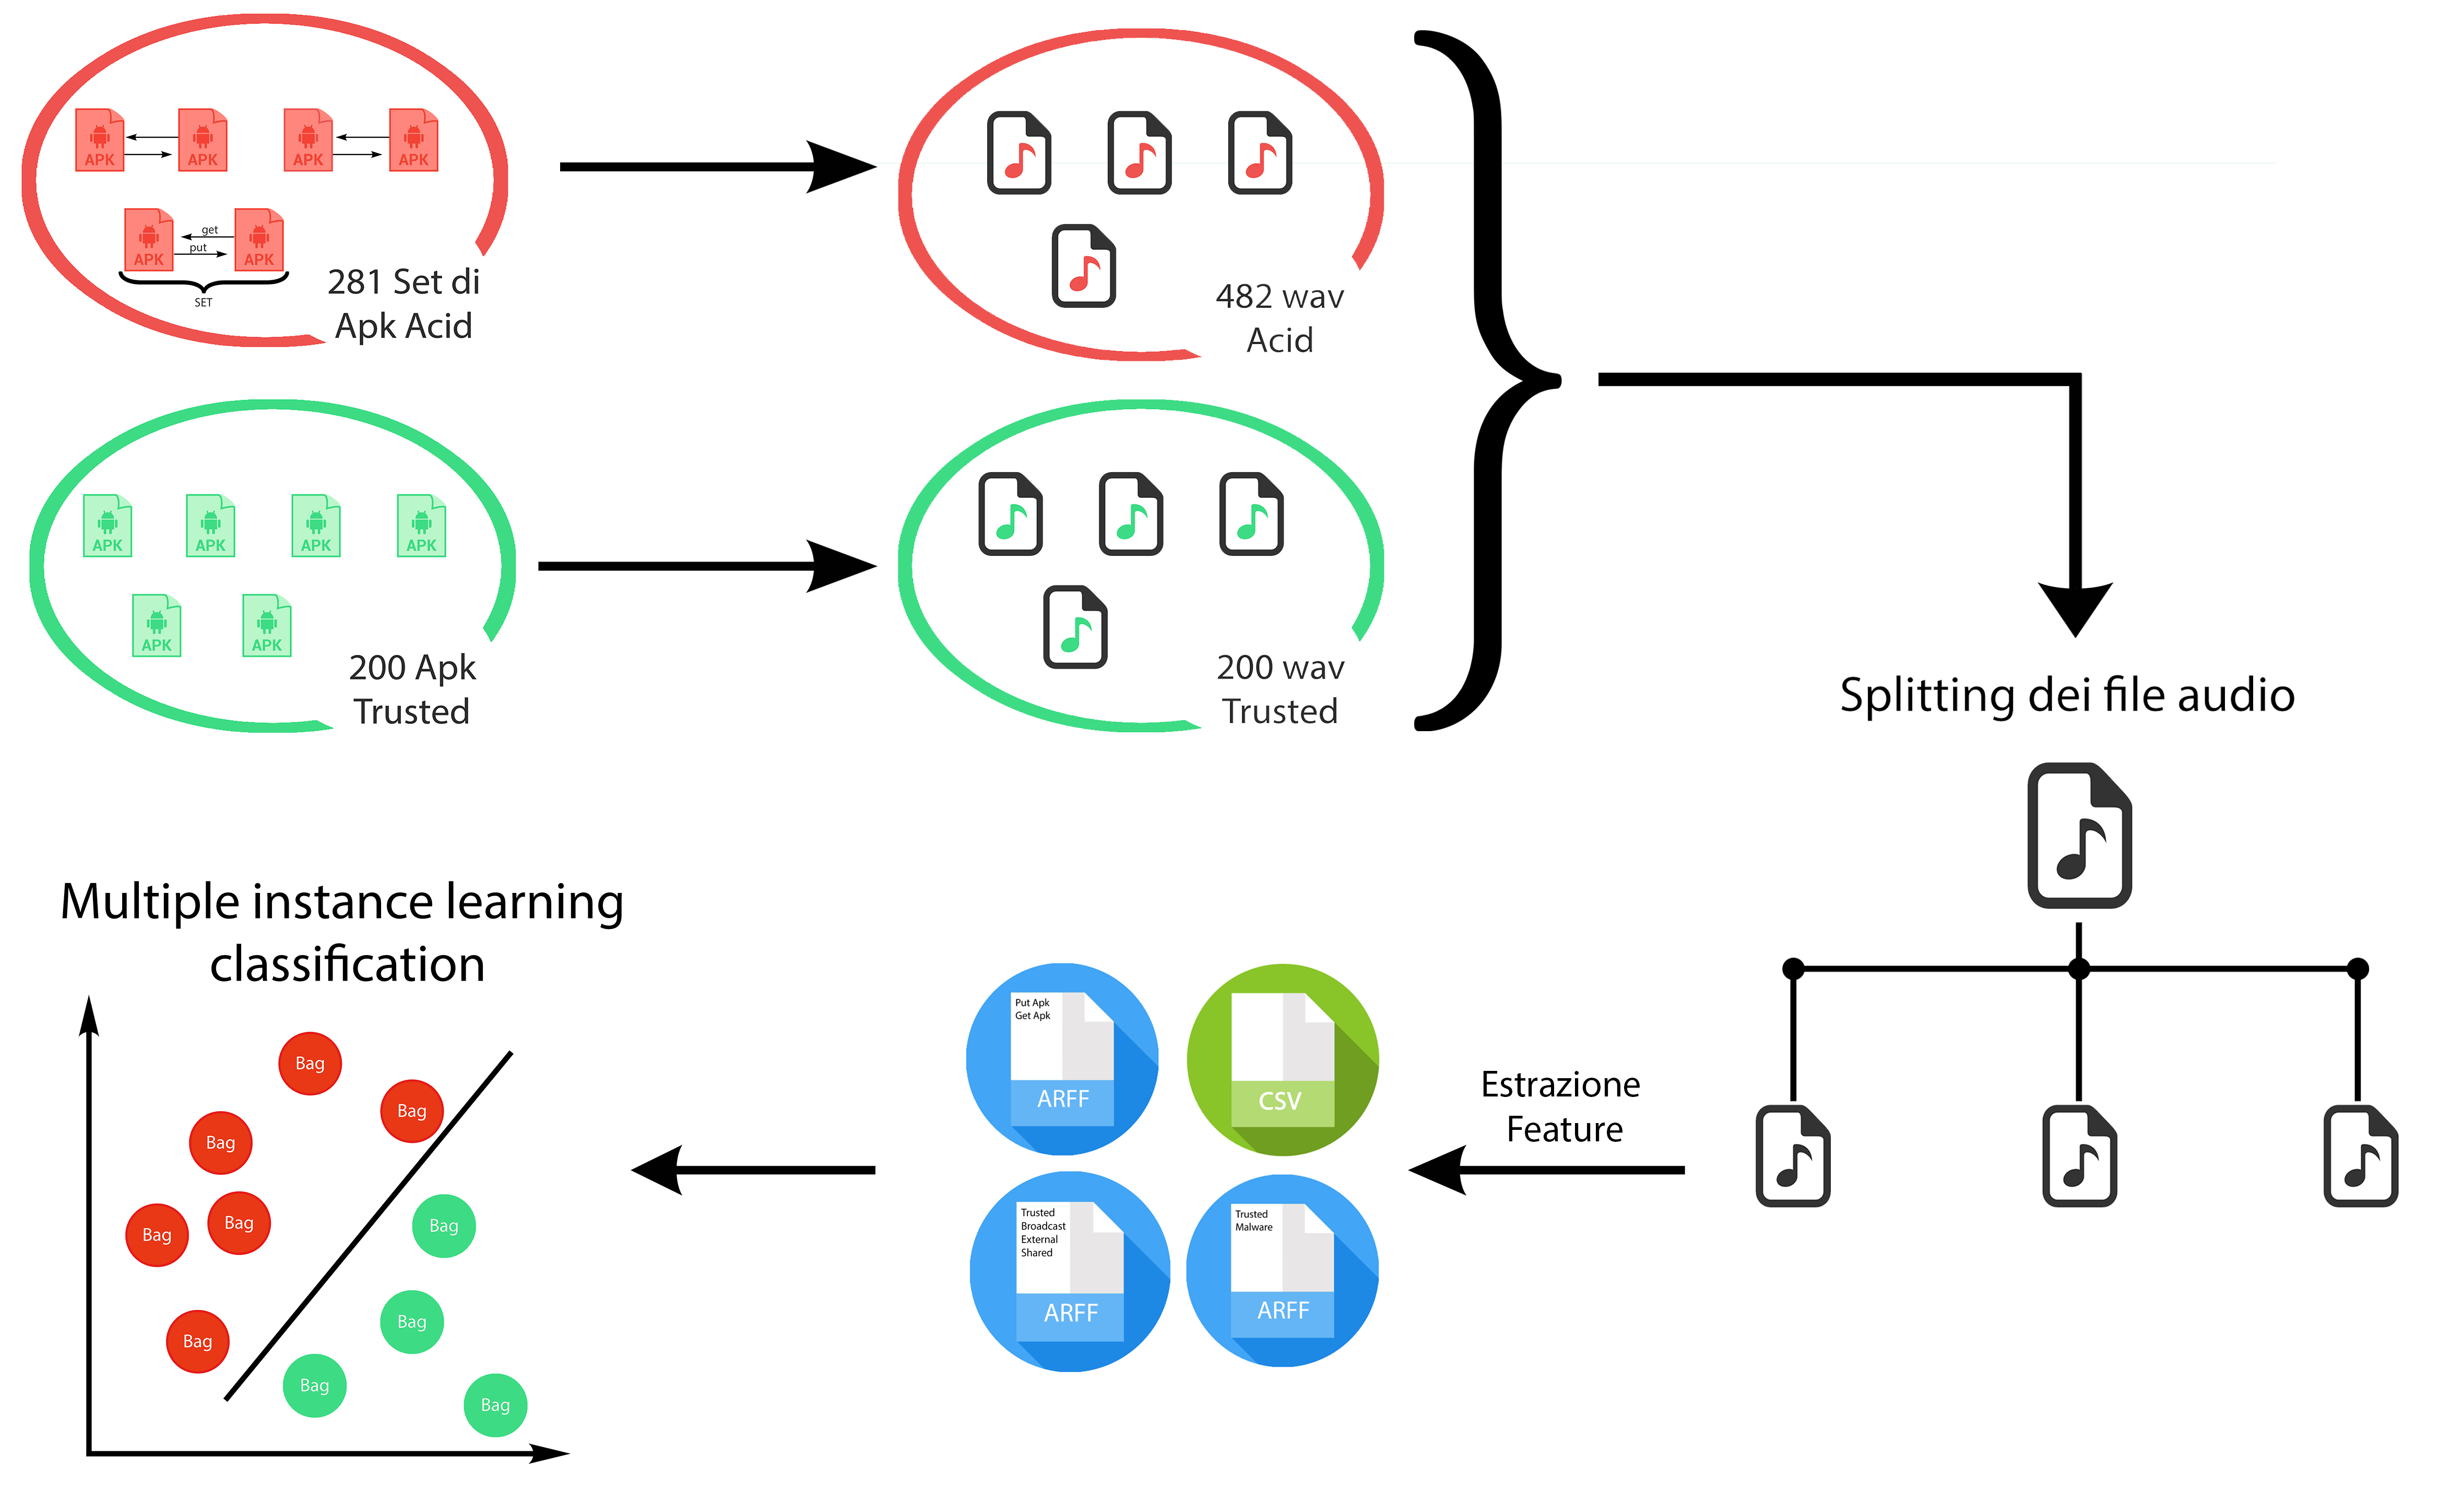
\includegraphics[width=0.9\linewidth]{imgs/capitolo4/all.png} 
    \caption{project}
    \label{fig:all}
\end{figure}
\FloatBarrier
\section{I software e i dataset}
In questo paragrafo esporremo dapprima tutti i software utilizzati nell'analisi e una breve panoramica sulle caratteristiche principali dei dataset utilizzati.  
\subsection{WEKA}
Acronimo di "Waikato Environment for Knowledge Analysis", è un software open source per il machine learning. Partendo da un dataset\footnote{Collezione di dati organizzati, la grandezza è data dal numero di righe.} è possibile applicarvi dei metodi di apprendimento automatico e di analizzarne il risultato è inolttre possibile attraverso l'utilizzo di questi metodi avere una previsione su nuovi set di dati. Per poter utilizzare gli algoritmi di classificazione del multiple instance learning bisogna importare i relativi package, attravero il tool "Package Manager" già presente di default nella schermata iniziale di weka. Figura \ref{fig:mil pckg}.
\begin{figure}[h]
\centering
    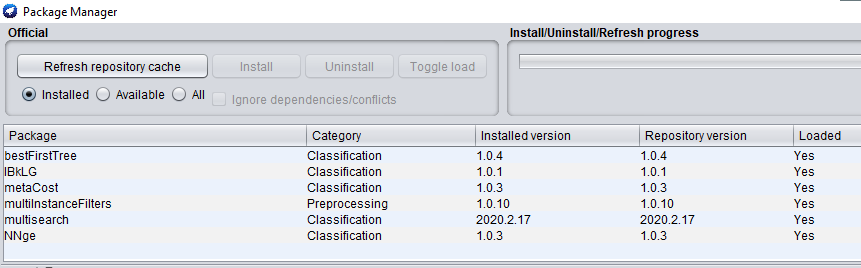
\includegraphics[width=0.9\linewidth]{imgs/capitolo4/packmil.png} 
    \caption{Imput Mil package in weka}
    \label{fig:mil pckg}
\end{figure}
\FloatBarrier
Una particolarità di questo software è l'utilizzo di dataset .arff 


\subsection{dataset.csv e dataset.arff}
I dataset utilizzati nel progetto sono dataset con estensione \textbf{.csv - Comma Separated Values}, questo è un formato di file di testo in cui ogni riga rappresenta un record della tabella. Ogni colonna invece rappresenta dei valori associati ad ogni record. le colonne sono separate da virgole, da qui il nome. In figura \ref{Fig:Datacsv} è possibile osservarne un esempio. 
\vspace{1em}
\newline
Il secondo tipo di dataset che abbiamo utilizzato sono file dati con estensione \textbf{.arff - Attribute Relationship File Format} come suggerisce il nome, questo formato di file organizza i dati seguendo una logica relazionale.
La formattazione del dataset utilizzato riguarda è stata svolta in ottica di una classificazione attraverso algoritmi di multiple instance learning, dunque si è reso necessario dover organizzare i dati in bag. L'inizializzazione del file, per una classificazione MIL\footnote{Mil - Multiple instance learning} può essere suddiviso in cinque componenti\cite{wekaDoc}:  
\begin{enumerate}
        \item Nella prima va sempre definita la relazione che lega i dati attraverso l'attributo \textbf{@relation} ed un nome che descriva quello che vogliamo predire.  
        
        \item Successivamente andranno inseriti gli identificativi delle bag, ovvero utilizzando \textbf{@attribute bag\_id \{...\}} si vanno ad inserire nelle parentesi graffe la lista di tutti gli identificative delle istanze della bag. Ogni identificativo va separato dall'altro tramite tramite l'utilizzo di una virgola. 
        
        \item Dopo si definiranno gli attributi della bag, per farlo si utilizzano\textbf{@attribute bag relational} per definire l'inizio della bag ed \textbf{@end bag}per definire la fine della bag. All'interno, tra i due attributi, vanno specificati gli attributi che compongono le istanze di una bag, ovvero le caratteristiche dei dati. Per farlo si utilizza ancora una volta l'identificativo \textbf{@attribute nome\_caratteriustica tipo\_caratteristica}. Il tipo di caratteristica può essere \textit{numeric} se il valore del dato è un numero intero, altrimeti \textbf{real} se il tipo di attributo è un numero reale altriment se il tipo di dato da rappresentare è una stringa scriveremo i valori ammissibili presenti tra parentesi graffe es. {\{yes, no\}} nel caso di un attributo booleano.
        
        \item A questo punto dobbiamo definire la classe che rappresenta una istanza. Per farlo inseriremo i valori tra parentesi graffe definendo l'attributo class come, \textbf{@attribute class {calss1, class2}}
        
        \item Infine attraverso a capo della key \textbf{@data} inseiremo il dataset correttamente formattato nel seguente modo: iesima bag\_id + ',' poi dovremmo definire tutte le istanze della bag. Una bag si definisca allinterno delle virgolette "...". All'intero delle virgolette inseiremo tutte le istanze ognuna della quali sara separata dal carattere speciale '$\backslash$n'. A loro volta ogni istanza è rappresentata dai diversi attributi, tanti quanti ne abbiamo definiti in precedenza, ogni attributo d'istanza è separato dall'altro tramite ','. Infine dopo la chiusura delle virgolette inseriamo la virgola e va definita la classe della bag. Ogni riga ha quindi la seguente formattazione:
        \\\footnotesize {
        bag\_id , " attr1Ist1, attr2Ist1, attr3Ist1 $\backslash$n attr1Ist2, attr2Ist2, attr3Ist2 $\backslash$n attr1Ist3, attr2Ist3, attr3Ist3 " , classe  }
    \end{enumerate}
\begin{figure}[h]
   \begin{minipage}{0.48\textwidth}
     \centering
     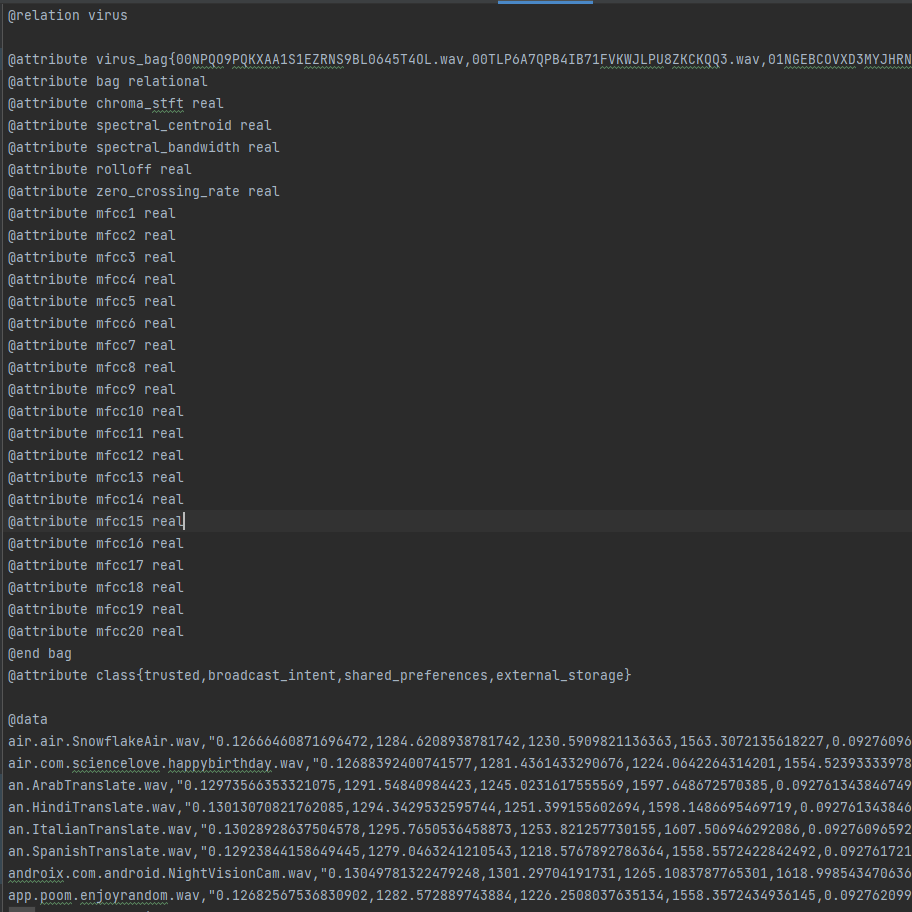
\includegraphics[width=0.85\linewidth]{imgs/capitolo4/ARFF.png}
     \caption{ARFF dataset for MIL}
     \label{Fig:Dataarff}
   \end{minipage}\hfill
   \begin{minipage}{0.48\textwidth}
     \centering
     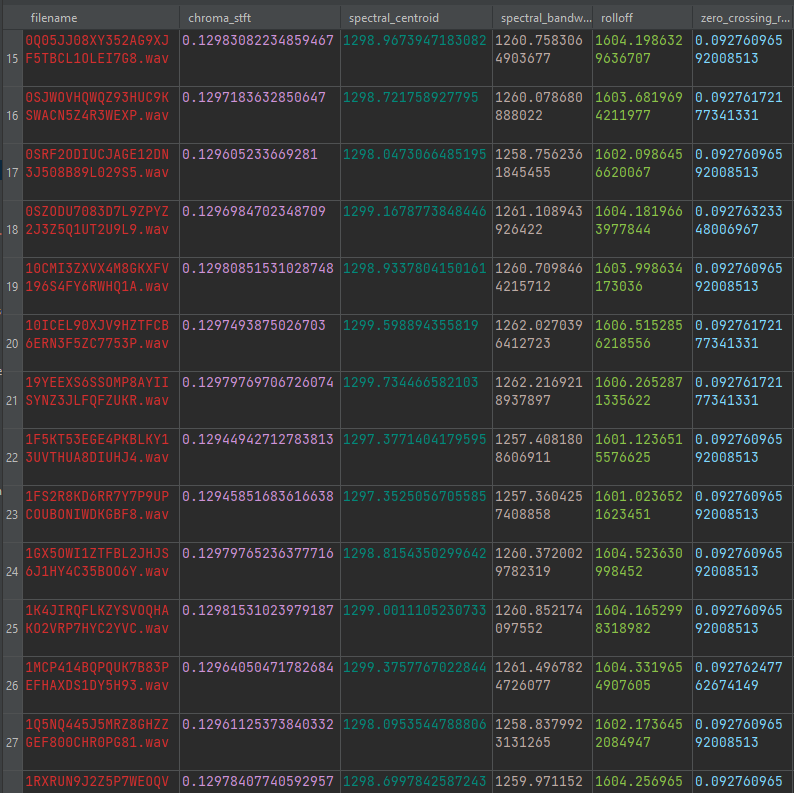
\includegraphics[width=0.85\linewidth]{imgs/capitolo4/csv.png}
     \caption{CSV file}
     \label{Fig:Datacsv}
   \end{minipage}
\end{figure}
\FloatBarrier 
\subsection{dataset di applicativi andorid}
Siamo partiti da due dataset di applicazioni apk. La prima conteneva un set di 200 applicazioni andorid non affette da malware che abbiamo definito il dataset come "trusted", il secondo dataset invece conteneva 241 applicazioni affette da malware abbiamo definito questo dataset come "Acid". TODO:...
\section{Elaborazione dei file audio}
In questo paragrafo descriveremo l'elaborazione dei file audio, coem sono stati generati e suddivisi.
